%!TEX root = ../main.tex
%% Chapter 4 - Experiments


\chapter{Experiments}
This chapter presents the practical part of the bachelor work.
% First, a general description of how the experiment organization is presented. TODO

Then, the choice of the different machines will be discussed in Section \ref{sec:preliminary}.
For this choice, different little benchmarks have been used, which will be discussed.
Then, the configuration of the different physical and virtual machines will be presented in details, in order for these experiments to be reproducible.
The configuration includes the software installation and the tuning of MySQL database.
Finally, the different tests and their results will be discussed.


%%--------------- section
\section{Description and procedure}
A TPC-C database benchmark has been chosen in order to evaluate the performance of OpenStack.
The OLTP-Bench project has been used to run TPC-C benchmark on the different physical and virtual machines running a MySQL server.
The virtual machines are created with different configurations (flavors, volume attached or not). 
It is expected to see the difference in performance for these different configurations and therefore the performance of OpenStack.
These results will be compared to the results obtained when running OLTP-Bench on the chosen physical machine (Section \ref{sec:preliminary} shows how this machine is chosen).

The tests are conducted in four different phases.
In the first phase, OLTP-Bench is run on the chosen physical machine.
In the second phase, it is run on virtual machines with different flavors.
The third phase is similar to the second one, except that a volume is attached to the virtual machine.
The last phase aims to test isolation, which is done by running OLTP-Bench on two different virtual machines at the same time.




%%---------------
%%--------------- section
%%---------------
\section{Preliminary}
\label{sec:preliminary}
Before beginning benchmarking with OLTP-Bench, we need to have a point of comparison, a machine with which we can compare all the results obtained. 
In order to choose this machine, the \textit{hdparm}\footnote{\url{http://linux.die.net/man/8/hdparm}} and \textit{Bandwidth}\footnote{\url{https://zsmith.co/bandwidth.html}} benchmark have been used. 
These two benchmarks will evaluate physical machine components (hard disk and memory).
Based on their results, a reference machine will be chosen and the experiments will be carried on.


\subsection{HDPARM Benchmark}
%%--------------- begin: HDPARM
\textit{Hdparm} is a command line program on Linux systems and offers a great number of parameters that let one test the hardware of a machine in details. 
It should be noted that the use of some parameters can damage a computer and therefore they have not been used for this experiment. 
Running the benchmark is pretty straightforward and is shown in Listing \ref{lst:lst_hdparm}.
In order to issue these commands, one must be root or use the command with \texttt{sudo}.

{
\singlespacing
\begin{lstlisting}[frame=single,language=bash,caption={hdparm commands},label={lst:lst_hdparm}]
#run on physical machines:
  $ hdparm -Tt /dev/sda1
#run on virtual machines:
  $ hdparm -Tt /dev/vda1
#run on virtual machines with a volume:
  $ hdparm -Tt /dev/vdb
\end{lstlisting}
}

The options \texttt{-Tt} instruct to benchmark the reading speed of the HDD and the reading speed of the memory (RAM) without accessing the HDD. 
The result returned by the benchmark is the reading average speed expressed in MB/s. 
The value returned by the option \texttt{T} is \textit{Timing cached reads} and measures the reading speed of the RAM and swap in case the memory is full. 
The value returned by the option \texttt{t} is \textit{Timing buffered disk reads} and measures the reading speed of the HDD in the specified partition.
The commands in Listing \ref{lst:lst_hdparm} were run six times and the average results are presented in Table \ref{table:hdparm_res_PM} for the physical machines. 

Based on the presented results, \texttt{compute2} shows the best performance regarding its hard drive, even if the difference with the two other machines is very small. 
Thereby, this machine was chosen as a compute node and block storage node for OpenStack.
Thus, \texttt{compute2} is the reference machine with which benchmark results will be compared to.
The \texttt{compute1} machine was chosen as a compute node, as it has the highest value regarding the cached reads.
The \texttt{machine4} is not part of the experiments, even if it was a potential candidate from the results obtained in Table \ref{table:hdparm_res_PM}.

\begin{table}[h]
	\centering
	\begin{tabular}{|m{6cm}|m{2.5cm}|m{2.5cm}|m{2.5cm}|}
		\hline
		& 
		\texttt{compute1} & %vm116
		\texttt{compute2} & %vm115
		\texttt{machine4} \\
		\hline
		\textbf{Buffered disk reads (MB/s)} & 
		120.65 & 
		134.06 & 
		124.86 \\
		\hline
		\textbf{Cached reads (MB/s)} &  
		15428.67 & 
		15327.23 & 
		15408.54 \\
		\hline
	\end{tabular}
	\caption{hdparm results for physical machines}
	\label{table:hdparm_res_PM}
\end{table}

The same procedure is applied to virtual machines.
For this, virtual machines were created on the two nodes: \texttt{compute1} and \texttt{compute2}.
We expect to obtain similar results as the virtual machines are using the same hardware as their host.
The results are presented in Table \ref{table:hdparm_res_VM} for the virtual machines with flavors \textit{large} and \textit{physical}. The case where a volume is attached to the virtual machine is also considered.

\begin{table}[h]
	\centering
	\begin{tabular}{|m{6.5cm}|m{1.5cm}|m{1.5cm}|m{1.5cm}|m{1.5cm}|}
		\hline
		\textbf{\textit{physical}} & 
		\texttt{vm1} & 
		\texttt{vm1bs} & 
		\texttt{vm2} & 
		\texttt{vm2bs} \\
		\hline
		\textbf{Buffered disk reads (MB/s)} & 
		126.61 & 
		110.8 & 
		117.58 & 
		320.44* \\
		\hline
		\textbf{Cached reads (MB/s)} &  
		14269.78 & 
		14223.5 & 
		15165.49 & 
		14890.86 \\
		\hline\hline
		\textbf{\textit{large}} & 
		\texttt{vm1} & 
		\texttt{vm1bs} & 
		\texttt{vm2} & 
		\texttt{vm2bs} \\
		\hline
		\textbf{Buffered disk reads (MB/s)} & 
		124.48 & 
		110.61 & 
		103.38 & 
		536.1* \\
		\hline
		\textbf{Cached reads (MB/s)} &  
		15520.6 & 
		15526.52 & 
		15372.97 & 
		15842.84 \\
		\hline
	\end{tabular}
	\caption{hdparm results for VMs}
	\label{table:hdparm_res_VM}
\end{table}

The results obtained with virtual machines are quite interesting.
Indeed, better results regarding HDD are obtained for \texttt{vm1} hosted on the less performant machine \texttt{compute1}, whereas poorer results are obtained for \texttt{vm2}.
The fact is that this benchmark is run on a short period of time (2-3 seconds) and 
it's difficult to evaluate hard disk and memory performance as they are always used by the system (some running processes can affect the results). 
Other runs showed lower performance results (around 105 MB/s) for \texttt{vm1} for example.
So, we can assume that both virtual machines (\texttt{vm1} and \texttt{vm2}) have quite similar performance and thus we expect to have quite similar results between them after running OLTP-Bench.
More interesting results are shown with values followed by a star (*). 
Indeed, they present quite high performance results when a volume (hosted on \texttt{compute2}) is attached to the virtual machine (also hosted on \texttt{compute2}).
When hdparm was performed, the timing buffered disk reads result increased between each run and did not stay stable like all other runs.
Thus, one can expect to observe a similar behavior when running OLTP-Bench.
As a result, \texttt{vm2} is chosen as the reference machine (for the virtual machines), as it presents better performance results regarding the cached reads.
%%--------------- end: HDPARM


%%--------------- begin: RAM bandwidth
\subsection{Bandwidth Benchmark}
We also benchmarked the RAM with an open source program called \textit{Bandwidth}. 
This artificial benchmark was run in order to be sure that the RAM of each machine has the same performance, as we would have expected from the output of hdparm shown in the previous section.
As we were only interested in the first outputs of Bandwidth, we did not run systematically the full test. Here is an excerpt of Sequential reads output from \texttt{vm2} with \textit{large} flavor after executing the command shown on the first line:

\begingroup
	\singlespacing
    \fontsize{10pt}{12pt}\selectfont
\begin{verbatim}
	$ sudo nice -n -2 ./bandwidth64
    ...
    Sequential read (64-bit LODSQ), size = 128 B, loops = 241172480, 5879.4 MB/s
    Sequential read (64-bit LODSQ), size = 256 B, loops = 174587904, 8523.1 MB/s
    Sequential read (64-bit LODSQ), size = 384 B, loops = 134566740, 9848.3 MB/s
    Sequential read (64-bit LODSQ), size = 512 B, loops = 109969408, 10736.3 MB/s
    Sequential read (64-bit LODSQ), size = 640 B, loops = 94056729, 11474.7 MB/s
    Sequential read (64-bit LODSQ), size = 768 B, loops = 80740044, 11823.8 MB/s
    Sequential read (64-bit LODSQ), size = 896 B, loops = 71752284, 12255.5 MB/s
    Sequential read (64-bit LODSQ), size = 1024 B, loops = 64028672, 12500.3 MB/s
    Sequential read (64-bit LODSQ), size = 1280 B, loops = 52952280, 12920.0 MB/s
    ...
\end{verbatim}
\endgroup

Similar results are obtained for each physical and virtual machines. 
As it was expected, the performance does not change too much and tend to stay the same on each machine.
%%--------------- end: RAM bandwidth

\subsection{OLTP-Bench configuration}
Now that we have our machines, we can begin to run OLTP-Bench on it. 
Before running the tests, the database has to be filled up with the different scale factor: 1, 16, 32, 64, 74, 84, 94, 104. 
To do this we must first create the appropriate databases: tpcc\_1, tpcc\_16\_ tpcc\_32, tpcc\_64, tpcc\_74, tpcc\_84, tpcc\_94, tpcc\_104. 
Then we can issue the command in Listing \ref{lst:lst_cmd_oltpbenchmark} from the terminal to fill up the databases.

{
\singlespacing
\begin{lstlisting}[frame=single,language=bash,caption={Database population command},label={lst:lst_cmd_oltpbenchmark}]
  $ ./oltpbenchmark -b tpcc -c config/tpcc_s1_t40_config.xml \
    --create=true --load=true
\end{lstlisting}
}

Listing \ref{lst:lst_oltp_config} shows an example of a configuration file for OLTP-Bench. 
This file specifies the connection details to access the database, then the scale factor and finally the workload. 
In the workload, only the number of terminals and the time the benchmark should last have been changed. 
Different configuration files were created in advance in order to facilitate the execution of the different benchmarks. 
In order to do this, all configuration files names are following a convention, in which we specify the scale factor number (s1 in our example) and the number of terminals (t40 in our example).
With this, a little bash script named \textit{oltpbench-run}\footnote{\url{https://github.com/nad0u/oltpbench-run}, 20.05.2015} 
has been created in order to launch one of the created configuration files by specifying the scale factor as an argument (see example in Listing \ref{lst:lst_cmd_oltpsh}).
It is possible to enter more than one argument, in case one wants to launch several benchmarks with different scale factors, one after another.

{
\singlespacing
\begin{lstlisting}[frame=single,language=bash,caption={Bash script for launching benchmarks},label={lst:lst_cmd_oltpsh}]
  $ ./oltpbench-run 1
\end{lstlisting}
}

The command in Listing \ref{lst:lst_cmd_oltpsh} will look for the configuration file corresponding to the scale factor 1 (s1) and to 40 terminals (t40), and run the benchmark twice, saving all the data in folders which will be compressed.
The number of terminals must be changed in the script, same goes for the machine name on which the benchmark is run.
As a side note, this script will not create folder to store the results, they have to be created in advance and be named as \texttt{results\_sX} (X is the scale factor number).

{
\singlespacing
\lstset{
    language=xml,
    tabsize=3,
    %frame=lines,
    caption=OLTP-Bench configuration file example,
    label=lst:lst_oltp_config,
    frame=single,
    rulesepcolor=\color{gray},
    xleftmargin=20pt,
    framexleftmargin=15pt,
    keywordstyle=\color{blue}\bf,
    commentstyle=\color{gray},
    stringstyle=\color{red},
    numbers=left,
    numberstyle=\tiny,
    numbersep=5pt,
    breaklines=true,
    showstringspaces=false,
    emph={
    	parameters,
    	driver,
    	dbtype,
    	DBUrl,
    	username,
    	password,
    	isolation,
    	scalefactor,
    	terminals,
    	works,
    	work,
    	time,
    	rate,
    	weights,
    	transactiontypes,
    	transactiontype,
    	name
    	},
    emphstyle={\color{magenta}}
    }
    \lstinputlisting{"source_code/tpcc_s1_t40_config.xml"}
}







%%---------------
%%--------------- section
%%---------------
\section{Software}
\label{sec:softwares}
The actual software and their configuration used in order to run the benchmark are presented in this section.

To run the benchmark we will be using the OLTP-Bench project, which can be cloned 
% (see Listing \ref{lst:lst_cmd_oltpb_cloning}) 
or downloaded from GitHub if Git is not installed on the system. 
OLTP-Bench is written in Java and need several sotfware to be installed in order to work (see Listing \ref{lst:lst_cmd_others_install}): 

{
\singlespacing
\begin{itemize}
\item \textit{OpenJDK}\footnote{\url{http://openjdk.java.net}}, an open source implementation of the Java Platform (version 1.7.0\_79)
\item \textit{Ant}\footnote{\url{http://ant.apache.org}} automates redundant operations in software development (version 1.9.3)
\item \textit{MySQL}, a database server (version 5.5.43)
\end{itemize}
}

After the installation, the OLTP-Bench system can be built with \textit{Ant}.

{
\singlespacing
\begin{lstlisting}[frame=single,language=bash,caption={Ant, Java and MySQL installation},label={lst:lst_cmd_others_install}]
  $ sudo apt-get install ant
  $ sudo apt-get install openjdk-7-jdk
  $ sudo apt-get install mysql-server
\end{lstlisting}
}

Instead of using the default configuration of MySQL, we will tune server parameters with the help of a script, 
named \texttt{mysql\_start.sh}, provided on the wiki page of the OLTP-Bench 
project\footnote{\url{http://oltpbenchmark.com/experiments/dbms_config/mysql_start.sh}}. 
This configuration is used for maximum performance. 
Before using the script, we need to create a new folder that will hold the database instead of the one used by default by MySQL. 
The new database location will be found in \texttt{/tmp/tpcc}. 
To prevent the \texttt{/tmp} folder to be cleaned after a reboot, we need to edit the file \texttt{/etc/default/rc5} and set \texttt{TMPTIME=-1}. 
Then we need to edit the \texttt{mysql\_start.sh} script accordingly by replacing the second line by \texttt{DATADIR=/tmp/tpcc}. 
Now we need to initialize the new MySQL data directory, shut down the current running MySQL service and start MySQL again with the script (see Listing \ref{lst:lst_cmd_mysql_start}).

{
\singlespacing
\begin{lstlisting}[frame=single,language=bash,caption={Ant, Java and MySQL installation},label={lst:lst_cmd_mysql_start}]
  $ sudo mysql_install_db --datadir=/tmp/tpcc --user=mysql
  $ sudo service mysql stop
  $ sudo ./mysql_start.sh
\end{lstlisting}
}

Afterwards, we are ready to start benchmarking. The different benchmarks are described in details in the four following sections.







%%---------------
%%--------------- section
%%---------------
\section{Phase 1 - Physical machine}
In order to have a point of comparison, the OLTP-Bench programm will be executed on the physical machine that performs the best regarding \texttt{hdparm} results, namely \texttt{compute2}.
Before running the tests, we will fill up the database with the different scale factors: 1, 16, 32, 64, 74, 84, 94, 104 (see Listing \ref{lst:lst_cmd_oltpbenchmark}). 
The size of each filled database is shown in Table \ref{table:tab_oltpb_scalefactor}.

\begin{table}[h]
	\centering
	\begin{tabular}{*{9}{|c}|}
		\hline
		\textbf{Database} & 
		1 & 
		16 & 
		32 & 
		64 & 
		74 & 
		84 & 
		94 &
		104 \\
		\hline
		\textbf{Size (in MB)} & 
		93.6 & 
		1922.9 & 
		3134.5 & 
		5603.2 & 
		6628.3 & 
		7381.6 & 
		8285.6 &
		9121.8 \\
		\hline
	\end{tabular}
	\caption{Database sizes}
	\label{table:tab_oltpb_scalefactor}
\end{table}

Once the databases populated, we can run the benchmarks by using the \texttt{oltpbench-run} script. 
In order to maximize performance, all the OpenStack services will be shut down during the tests. 
Moreover, the machines will be rebooted after each scale factor test. 
It has to be noted that after each run, the database will grow as many writes occur. 
Despite this, the databases will not be refilled after each test. 
Also, these tests were done with 40 terminals. 
The benchmark has been excuted two times, each run lasting 1800 seconds.

\begin{figure}[h]
	\centering
	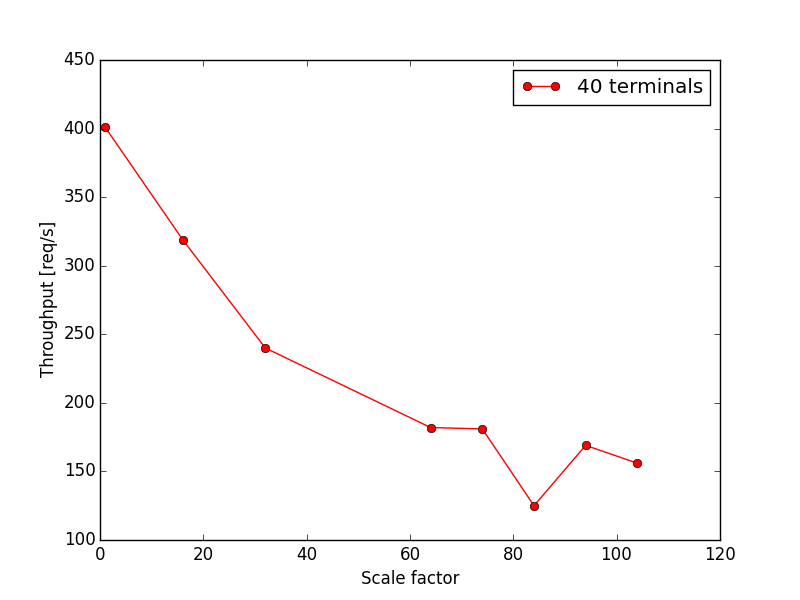
\includegraphics[scale=0.5]{figures/results/ph115_t40.png}
	\caption{\texttt{compute2} results}
	\label{fig:ph115_t40}
\end{figure}

As it can be seen in Figure \ref{fig:ph115_t40}, as the scale factor increases the throughput decreases. 
This behaviour is normal, as with a larger scale factor the database becomes bigger, and thus there is a lot more data to process and this will reduce the throughput of the system. 
For scale factor 84, we can see a little drop in the throughput. 

The throughput represented in the graph is computed by taking the 3600 throughput values ($2\times1800$ output values) of the OLTP-Bench output and calculating the first quartile $Q1$ and the third quartile $Q3$. 
The difference of $Q3$ and $Q1$ corresponds to the the interquartile range (IQR), which is a measure of statistical dispersion (see Equation \ref{eq:eq_iqr}). 
The final throughput will be computed by taking only output values between $Q1$ and $Q3$ included (or values in the IQR) and compute the median of these values.

\begin{equation}
   IQR = Q3 - Q1
   \label{eq:eq_iqr}
\end{equation}





%%---------------
%%--------------- section
%%---------------
\section{Phase 2 - Virtual machine without volume}
\label{section:phase2}

As for the physical machine, databases will be created and populated before running OLTP-Bench. 
Since the process of filling the databases is very long (especially for large scale factors), snapshots of the virtual machine are taken.
All databases cannot be stored in only one virtual machine, which is made of a disk of 30 GB (as defined in Table \ref{table:flavors_list_2}).
So there will be two snapshots: one with databases with scale factors from 1 to 74, and the second one with the rest.
These snapshots are named \textit{snap\_trusty\_16-74\_oltpsh\_} and \textit{snap\_trusty\_84-104\_oltpsh\_} respectively on the web interface of OpenStack.
This way, it will be easy to destroy and create a new virtual machine with a different flavor and have the populated database ready to be used.

For this phase, OLTP-Bench was run on two different virtual machines with different flavors, \texttt{vm2} \textit{large} and \texttt{vm2} \textit{physical}. 
For the virtual machine with \textit{large} flavor, OLTP-Bench was run with two different values for the terminals parameter: 1 and 40.
In the case of the physical flavor, OLTP-Bench was run only with 40 terminals.
Another thing to take care before running the benchmark on any \textit{large} flavor virtual machine: it is important to change the buffer pool size in the \texttt{mysql\_start} script. 
Otherwise, this will produce an error as the buffer pool is as big as the RAM on the virtual machine.
The new value is set to 6G instead of 8G: \texttt{--innodb-buffer-pool-size=6G}.

\begin{figure}[h]
	\begin{minipage}{.5\textwidth}
		\centering
		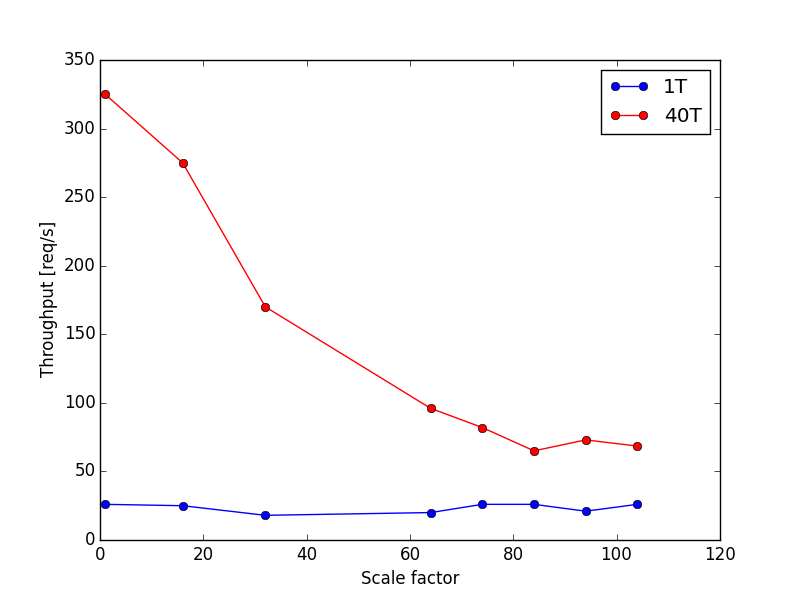
\includegraphics[scale=0.42]{figures/results/vm115_large_wobs.png}
		% \caption{\texttt{vm2} results for large flavor}
		\captionof{figure}{\texttt{vm2} results for large flavor}
		\label{fig:vm115_large_wobs}
	\end{minipage}
	\begin{minipage}{.5\textwidth}
		\centering
		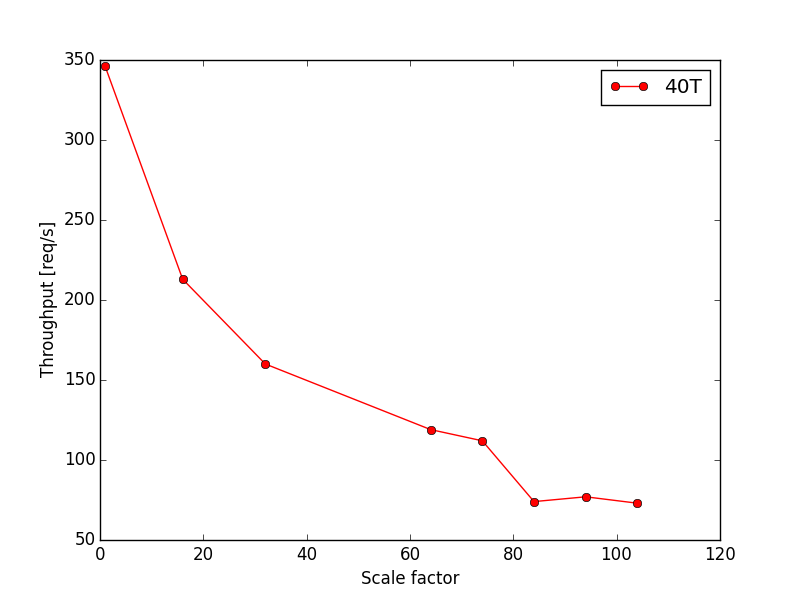
\includegraphics[scale=0.42]{figures/results/vm115_physical_wobs.png}
		% \caption{\texttt{vm2} results for physical flavor}
		\captionof{figure}{\texttt{vm2} results for physical flavor}
		\label{fig:vm115_physical_wobs}
	\end{minipage}
\end{figure}

As it can be seen in Figure \ref{fig:vm115_large_wobs} and \ref{fig:vm115_physical_wobs}, the throughputs with 40 terminals are quite similar between the \textit{large} and \textit{physical} flavors. 
However, with scale factor 16, we observe a greater throughput loss with the \textit{physical} flavor compared to the \textit{large} flavor. 
Also, like with the results on \texttt{compute2}, we observe again a drop at scale factor 84, especially with the \textit{physical} flavor. 
It seems to be a coincidence, because an analysis of the data (plotting througput over time in seconds) shows that the benchmark crashes at some point (i.e. there is 0 values for quite some time).
This behavior appears quite frequently over all the different runs made, but in some case, like with scale factor 84, it has a greater impact.
An example of such a crash is shown in Figure \ref{fig:vm115_physical_wobs_crash} (blue corresponds to the first run and red to the seconde run).
The crash begins after 450 seconds and lasts 150 seconds approximately.

\begin{figure}[h]
	\centering
	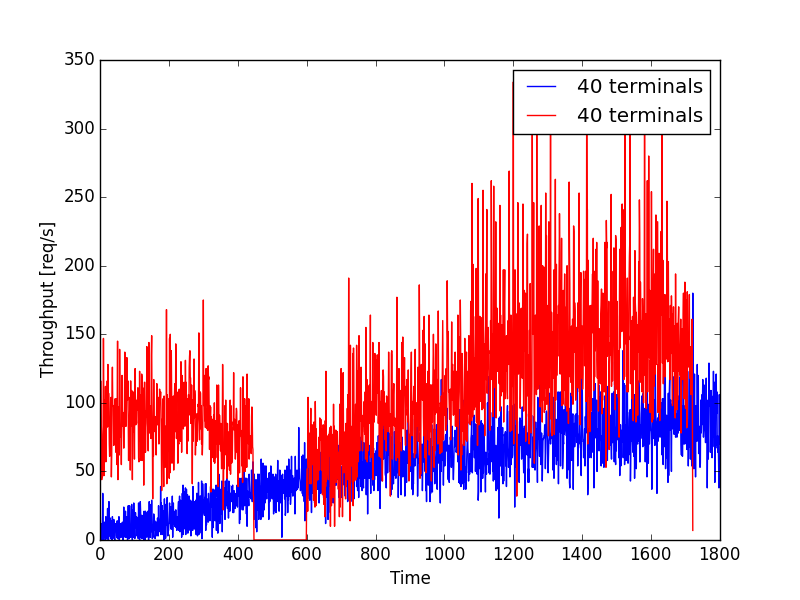
\includegraphics[scale=0.5]{figures/results/vm115_physical_wobs_crash.png}
	\caption{Crash on \texttt{vm2} physical (scale factor 84)}
	\label{fig:vm115_physical_wobs_crash}
\end{figure}

Concerning the results obtained with 1 terminal, we can see that they are quite constant.
It can be interesting to run the same benchmark with different values for the number of terminals in order to see where we have better performance.

Finally, one can observe that in general, better performances are achieved on \texttt{compute2} with a peak at 400 req/s for scale factor 1.
So, for now, OpenStack does not seem to beat the performance of a physical machine.






%%---------------
%%--------------- section
%%---------------
\section{Phase 3 - Virtual machine with volume}

During this phase, the same tests as in Section \ref{section:phase2} will be run, but instead of using the ephemeral storage that comes with each virtual machine, we will be using the OpenStack service for storage, known as Block Storage. 
The Block Storage service lets us create a volume that can be seen as an external HDD that is attached to a computer. 
So basically, instead of storing the database in the default HDD of the virtual machine, it will be stored on the attached volume.

Before beginning the tests, some changes have to be made in order for everything to work. 
After changing the database location (moved on the attached volume), the AppArmor application will prevent MySQL to start, if it is not well configured. 
This application is installed by default on Ubuntu system, and is \textquote{\textit{a kernel-integrated application security system that controls how applications can access the file system}}
\footnote{\url{https://blogs.oracle.
com/jsmyth/entry/apparmor_and_mysql}, 17.02.2015}. 
As we are going to move the database on the attached volume, this new location must be known by the AppArmor application. 
Until now we did not need to make any changes, as by default MySQL has access to the \texttt{/tmp} folder on Unix based systems
\footnote{\url{http://dev.mysql.com/doc/refman/5.7/en/temporary-files.html}, 17.02.2015}. 
To attach a volume to the virtual machine, we need to create a new directory \texttt{/myspace} on which it will be mounted. 
The different commands to mount and move the database are shown in Listing \ref{lst:lst_cmd_mount_movedb}.

{
\singlespacing
\begin{lstlisting}[frame=single,language=bash,caption={Mount volume and move database},label={lst:lst_cmd_mount_movedb}]
  # Format the volume if it's not already done:
  $ mkfs -t ext4 /dev/vdb

  # Mount the volume on the created folder:
  $ mount /dev/vdb /myspace

  # Copy the databases and keep the same permissions:
  $ cp -rp /tmp/tpcc /myspace/
\end{lstlisting}
}

Once the data have been moved, we can shutdown MySQL and add the new database location to AppArmor (see Listing \ref{lst:lst_apparmor}). 
After reloading AppArmor, we also need to change the \texttt{DATADIR} variable in the \texttt{mysql\_start} script used for tunning MySQL. 
Instead of \texttt{DATADIR=/tmp/tpcc}, we have \texttt{DATADIR=/myspace/tpcc}. 
Now, we are ready to benchmark OpenStack using attached volumes to virtual machines.

{
\singlespacing
\begin{lstlisting}[frame=single,language=bash,caption={Configure AppArmor},label={lst:lst_apparmor}]
  # Add these two lines to /etc/apparmor.d/usr.sbin.mysqld
  /myspace/tpcc/ r,
  /myspace/tpcc/** rwk,

  # Reload AppArmor
  $ /etc/init.d/apparmor reload
\end{lstlisting}
}

For this part of the experiment, we wanted to see if the use of volumes attached to virtual machines can affect the performance, as it was observed when running \texttt{hdparm}. 
In particular, we want to see what happens when we have both the virtual machine and the volume hosted on the same physical machine (on \texttt{compute2} in our case) and when we have a virtual machine hosted on \texttt{compute1} and the volume hosted on \texttt{compute2}.

\begin{figure}[h]
	\begin{minipage}{.5\textwidth}
		\centering
		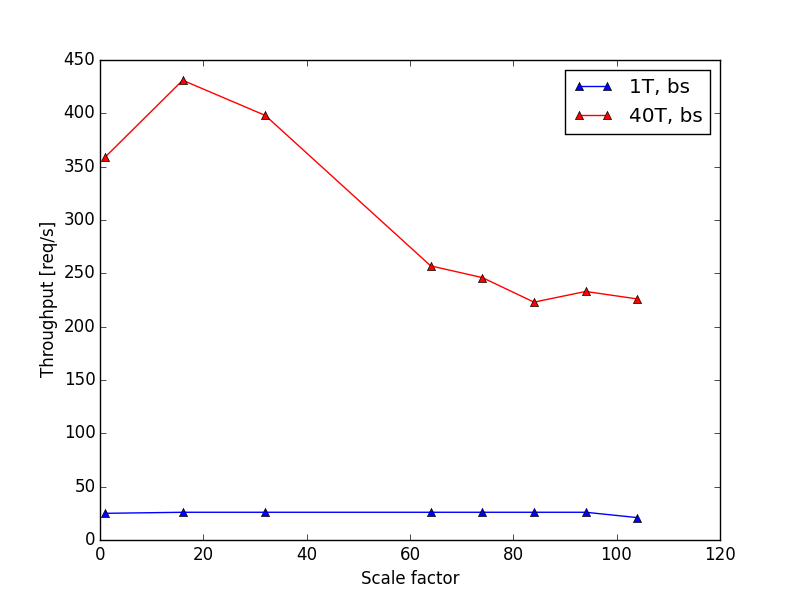
\includegraphics[scale=0.42]{figures/results/vm115_large_wbs.png}
		\captionof{figure}{\texttt{vm2bs} results for large flavor}
		\label{fig:vm115_large_wbs}
	\end{minipage}
	\begin{minipage}{.5\textwidth}
		\centering
		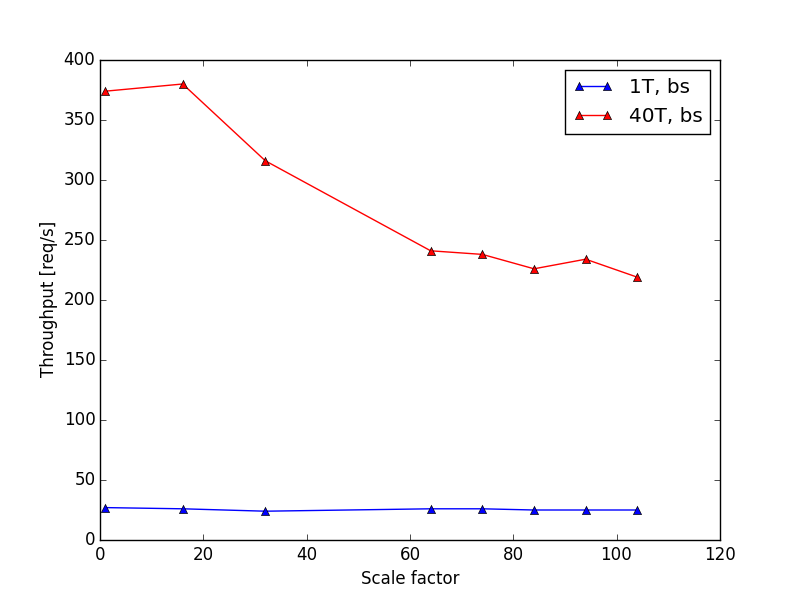
\includegraphics[scale=0.42]{figures/results/vm116_large_wbs.png}
		\captionof{figure}{\texttt{vm1bs} results for large flavor}
		\label{fig:vm116_large_wbs}
	\end{minipage}
\end{figure}

Like before, \textit{large} and \textit{physical} flavor will be used, and in the case of \textit{large} flavor, the benchmark will be run with 1 and 40 terminals. 
We will first discuss the case of \textit{large} flavor, whose results are shown in Figures \ref{fig:vm115_large_wbs} and \ref{fig:vm116_large_wbs}.
At first glance, we can see that both graphs have the same shape. However, this shape differs from the results obtained in Phase 2. 
In the case of 40 terminals, we see that the throughput increases from scale factor 1 to 16, instead of decreasing like before. 
Moreover, in the case of scale factor 1, we can see that the throughput is at least around 350 req/s and goes up to around 430 req/s in the case \texttt{vm2bs}.
Thus, compared to \texttt{compute2}, we can reach a higher throughput.

For the other scale factors, one can observe that the throughput decreases like previous results in Phase 2, except that at the end (scale factor 104), the throughput stagnates at a higher level around 225 req/s instead of 75 req/s in results obtained in Phase 2. 
In fact, the throughput never goes below 200 req/s. 
Most of the results lie between 200 req/s and 260 req/s, which is clearly better than results obtained in Phase 2, and even better that the results obtained in Phase 1 where most of the results are below 200 req/s. 
Finally, as to be expected, the results for 1 terminal are constant and there is no higher throughput as there is only one client interacting with the database. 

Now, comparing \texttt{vm2bs} and \texttt{vm1bs} results, we see that we obtain slightly better performance results for \texttt{vm2bs}, especially for scale factors 16 and 32. 
So one can say that having an attached volume hosted on the same physical machine as the virtual machine potentially increases the performance in the case of \textit{large} flavor.

For the case of \textit{physical} flavor, one can observe a similar shape as we had in Figures \ref{fig:vm115_large_wbs} and \ref{fig:vm116_large_wbs}, except that the throuhput drops rapidly under 300 req/s for scale factor 32.
And as expected, the performance is way better than what was obtained in Phase 2 (see Figure \ref{fig:vm115_large_wobs}). 
Indeed, throughputs are always above 200 req/s.

\begin{figure}[h]
	\begin{minipage}{.5\textwidth}
		\centering
		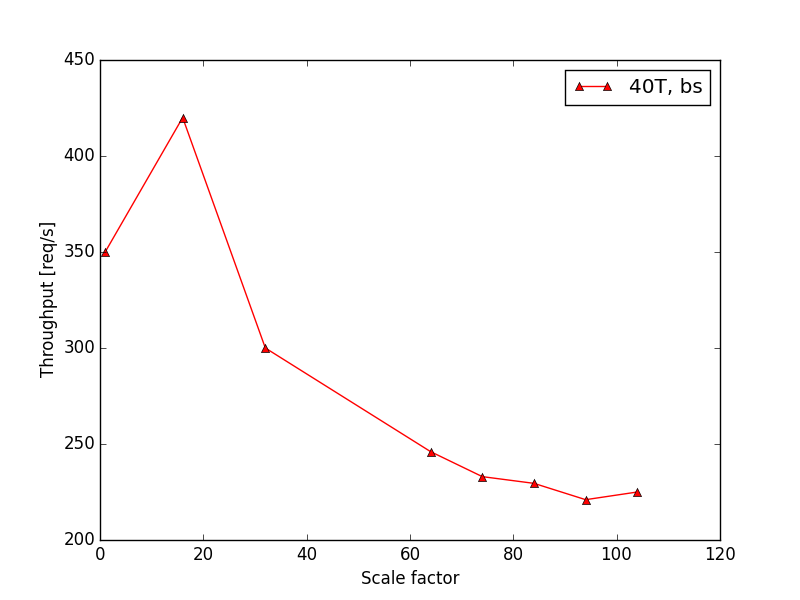
\includegraphics[scale=0.42]{figures/results/vm115_physical_wbs.png}
		\captionof{figure}{\texttt{vm2bs} results for physical flavor}
		\label{fig:vm115_physical_wbs}
	\end{minipage}
	\begin{minipage}{.5\textwidth}
		\centering
		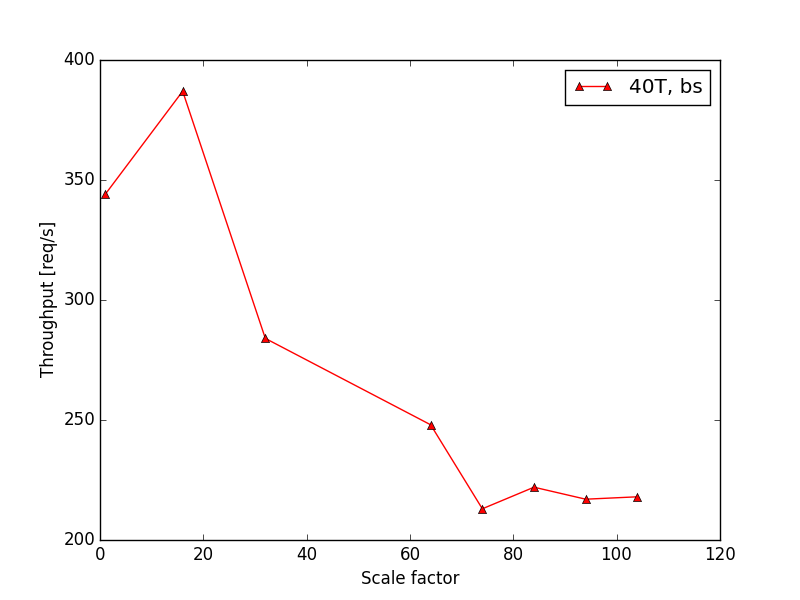
\includegraphics[scale=0.42]{figures/results/vm116_physical_wbs.png}
		\captionof{figure}{\texttt{vm1bs} results for physical flavor}
		\label{fig:vm116_physical_wbs}
	\end{minipage}
\end{figure}


Finally, as we can see, there is very little difference in performance between \textit{large} and \textit{physical} flavor when a volume is attached to the virtual machine. 
However, we obtain better performance compared to virtual machines without volume (see Figures \ref{fig:vm115_large_wobs} and \ref{fig:vm115_physical_wobs}). 
To conclude, we can say that having a volume attached to a virtual machine really improve the overall performance of the system.
Apparently, OpenStack is doing a great job with volumes management.




%%---------------
%%--------------- section
%%---------------
\section{Phase 4 - Virtual machines isolation}

As a final step for this project, we wanted to test isolation between the virtual machines.
Indeed, when several virtual machines are hosted on the same physical machine, they have to share the available hardware components (i.e. CPU, HDD, RAM) of the host.
Testing isolation allows us to verify that a virtual machine is not interfering (or not interfering too much) with another virtual machine running on the same host. 
It must also be the case when two virtual machines are running on two different hosts. 
Thus, a good isolation allows to keep individual performance of each virtual machine more or less intact.
The isolation is particularily important in \textit{Cloud Computing} as each hardware resource can be rented on demand. 
The customer that rented a virtual machine expects it to run at full power (the power he paid for), and so other virtual machines should not interfere with the rented one.

\begin{figure}[h]
	\centering
	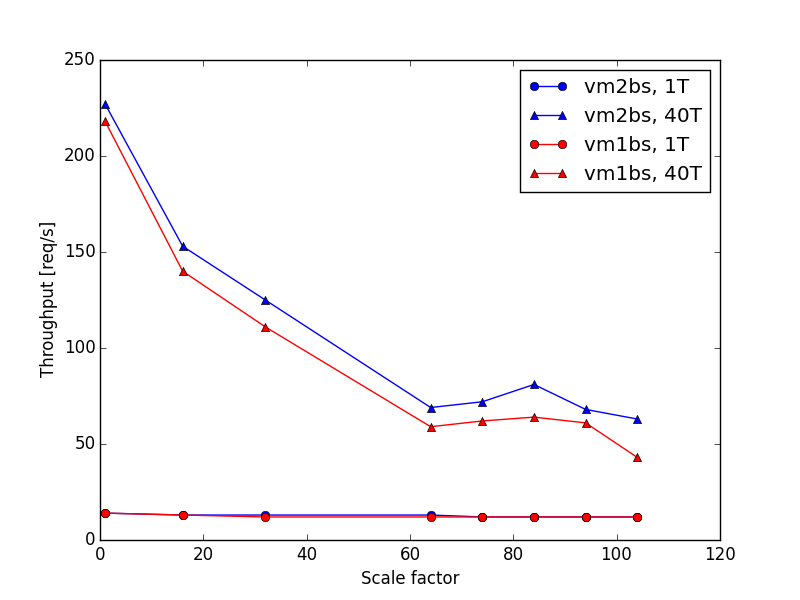
\includegraphics[scale=0.5]{figures/results/vm_large_iso.png}
	\caption{\texttt{vm1} (in red) and \texttt{vm2} (in blue) results for large flavor}
	\label{fig:vm_large_iso}
\end{figure}

In order to test isolation, we will consider the case where we have two virtual machines, \texttt{vm1} and \texttt{vm2}, running on two different physical machines, \texttt{compute1} and \texttt{compute2} respectively. 
Both virtual machines are created with \textit{large} flavor and have a volume (hosted on \textit{compute2}) attached to them. 
OLTP-Bench is executed at the same time on both virtual machines. 
As before, we are considering two different number of terminals: 1 and 40. 
The results of the experiments are shown in Figure \ref{fig:vm_large_iso}.

Unfortunately, this test does not return good results.
Indeed, almost all throughput lie below 200 req/s, which is clearly worse than all results obtained until now.
This can be explained by the fact that we do not have a dedicated machine for managing the volumes, a Block Storage node, in our OpenStack architecture.
This means that the two virtual machines try to access the same physical hard drive (where the database resides) during the benchmark, even if there are two logical volumes.

In order to better test isolation, one must consider having a dedicated machine for managing volume instead.
One can also try to run the same benchmark, without using volumes.
But as Phase 3 shown that better performance can be achieved by attaching volumes to the virtual machines, it seems logical to test isolation with volume also.

